\documentclass[11pt,conference,compsocconf]{IEEEtran}
\usepackage{tikz}
\usepackage{amsmath}
\usepackage{amssymb}
\usepackage{amsthm}
\usepackage{bm}
\usepackage[linesnumbered]{algorithm2e}
\makeatletter
\renewcommand{\@algocf@capt@plain}{above}
\makeatother
\usepackage[colorlinks,urlcolor=blue,citecolor=hotpink,linkcolor=blue]{hyperref}
\usetikzlibrary{decorations.pathreplacing}
\usetikzlibrary{arrows}
\usetikzlibrary{snakes}
\usetikzlibrary{calc}
\let\emptyset\varnothing
\definecolor{hotpink}{rgb}{0.9,0,0.5}
\definecolor{deepgray}{gray}{0.35}
\definecolor{deepgray2}{gray}{0.25}
\definecolor{deepgray3}{gray}{0.10}
\definecolor{lightgray}{gray}{0.95}
\definecolor{lightgray2}{gray}{0.85}
\definecolor{purple1}{RGB}{239,229,244}
\definecolor{purple2}{RGB}{216,191,216}
\definecolor{lightblue}{rgb}{0.73,0.33,0.83}
\definecolor{lightpurple}{rgb}{.8,.2,.8}
\definecolor{textcolor}{rgb}{0,0,5}
\definecolor{blue1}{RGB}{187,217,238}
\definecolor{blue2}{RGB}{235,244,250}
\definecolor{yellow1}{RGB}{255,249,234}
\definecolor{blue3}{RGB}{63,40,96}
\definecolor{red1}{RGB}{255, 102, 102}
\definecolor{green1}{RGB}{102, 255, 102}
\newtheorem{lemma}{Lemma}
\newtheorem{thm}{Theorem}
\theoremstyle{definition}
\def\proof{\par{\bf Proof}. \ignorespaces}
\def\qedsymbol{\vbox{\hrule\hbox{%
                     \vrule height1.3ex\hskip0.8ex\vrule}\hrule}}
\def\endproof{\qquad\qedsymbol\medskip\par}

% Some very useful LaTeX packages include:
% (uncomment the ones you want to load)


% *** MISC UTILITY PACKAGES ***
%
%\usepackage{ifpdf}
% Heiko Oberdiek's ifpdf.sty is very useful if you need conditional
% compilation based on whether the output is pdf or dvi.
% usage:
% \ifpdf
%   % pdf code
% \else
%   % dvi code
% \fi
% The latest version of ifpdf.sty can be obtained from:
% http://www.ctan.org/tex-archive/macros/latex/contrib/oberdiek/
% Also, note that IEEEtran.cls V1.7 and later provides a builtin
% \ifCLASSINFOpdf conditional that works the same way.
% When switching from latex to pdflatex and vice-versa, the compiler may
% have to be run twice to clear warning/error messages.

% *** CITATION PACKAGES ***
%
\usepackage{cite}
% cite.sty was written by Donald Arseneau
% V1.6 and later of IEEEtran pre-defines the format of the cite.sty package
% \cite{} output to follow that of IEEE. Loading the cite package will
% result in citation numbers being automatically sorted and properly
% "compressed/ranged". e.g., [1], [9], [2], [7], [5], [6] without using
% cite.sty will become [1], [2], [5]--[7], [9] using cite.sty. cite.sty's
% \cite will automatically add leading space, if needed. Use cite.sty's
% noadjust option (cite.sty V3.8 and later) if you want to turn this off.
% cite.sty is already installed on most LaTeX systems. Be sure and use
% version 4.0 (2003-05-27) and later if using hyperref.sty. cite.sty does
% not currently provide for hyperlinked citations.
% The latest version can be obtained at:
% http://www.ctan.org/tex-archive/macros/latex/contrib/cite/
% The documentation is contained in the cite.sty file itself.

% *** GRAPHICS RELATED PACKAGES ***
%
\ifCLASSINFOpdf
  % \usepackage[pdftex]{graphicx}
  % declare the path(s) where your graphic files are
  % \graphicspath{{../pdf/}{../jpeg/}}
  % and their extensions so you won't have to specify these with
  % every instance of \includegraphics
  % \DeclareGraphicsExtensions{.pdf,.jpeg,.png}
\else
  % or other class option (dvipsone, dvipdf, if not using dvips). graphicx
  % will default to the driver specified in the system graphics.cfg if no
  % driver is specified.
  % \usepackage[dvips]{graphicx}
  % declare the path(s) where your graphic files are
  % \graphicspath{{../eps/}}
  % and their extensions so you won't have to specify these with
  % every instance of \includegraphics
  % \DeclareGraphicsExtensions{.eps}
\fi

\usepackage{url}
% correct bad hyphenation here
\hyphenation{op-tical net-works semi-conduc-tor}


\begin{document}
%
% paper title
% can use linebreaks \\ within to get better formatting as desired
\title{An Algorithm for Searching Evolving Graphs in Linear Algebraic Language}

% author names and affiliations
% use a multiple column layout for up to two different
% affiliations
% \and

\author{
\IEEEauthorblockN{Jiahao Chen}
\IEEEauthorblockA{ Computer Science and Artificial Intelligence Laboratory,\\
Massachusetts Institute of Technology,\\
Massachusetts, 02139-4307,USA\\
jiahao@mit.edu}
\and
\IEEEauthorblockN{Weijian Zhang}
\IEEEauthorblockA{School of Mathematics,\\
University of Manchester,\\
Manchester, M13 9PL, England\\
weijian.zhang@manchester.ac.uk}
}

\maketitle

\begin{abstract}
  % A generalization of the breadth-first search (BFS) algorithm on evolving graphs is
  % discussed.
  % The representation of this algorithm
  % as algebraic operations is investigated.
  % The duality of the vector-matrix multiplication
  % and a BFS step is extended to the fact that a block vector-matrix multiplication
  % is dual with the evolving-graph BFS.
  % It is found that the algebraic representation allows for flexible forward and backward searching and can be used for mining citation networks.
A generalized breadth-first search (BFS) algorithm is presented for
searching evolving graphs.
The method is described in both graph and linear algebra notation and
the two algorithms are shown to be equivalent.
A preliminary discussion on mining citation networks is also presented.
\end{abstract}

\begin{IEEEkeywords}
~Evolving graph; complex network; breadth first search; data mining.
\end{IEEEkeywords}

% For peer review papers, you can put extra information on the cover
% page as needed:
% \ifCLASSOPTIONpeerreview
%\begin{center} \bfseries EDICS Category: 3-BBND \end{center}
% \fi
%
% For peerreview papers, this IEEEtran command inserts a page break and
% creates the second title. It will be ignored for other modes.
\IEEEpeerreviewmaketitle

\section{Introduction}

Let's imagine a game played by three people
$A$, $B$, and $C$. Suppose each of them has a piece of information,
say $X$, $Y$, and $Z$ respectively. The goal of the game is
to get information from other people as much as possible.
Suppose $A$ talks to $B$ first and then $B$ talks to $C$,
then $C$ may has all three pieces of information $X$, $Y$, and $Z$ even
if $C$ has never talked to $A$.
However, if $B$ talks to $C$ first and then $A$ talks to $B$, then
no matter how smart $C$ is, $C$ can never get information
$X$.  Time is an important factor for information flow.

We can analyze the spread of information between $A$, $B$, and $C$
as a process on a graph that changes over time.
Such graphs are known as evolving graphs.
% Evolving graphs are models to study this kind of scenario where the
% interrelations between entities are time-dependent.
% We assume that the reader is familiar with the basic graph terminology.
% All the necessary material can be found in}.
We follow the notation of (static) graphs in \cite{even12,kegi11}.
In general, a evolving graph $G(t) = (V(t), E(t))$ is  a graph where the node set
and edge set are functions of time $t$.
However, in different literature the term ``evolving graph'' has been
used to refer to slightly different models.
 Flajolet et al. \cite{fkp89} use the term to mean the evolution of random graphs.
Bahmani et al. \cite{bkmu12} use the term to mean a sequence of graphs where
the difference between two consecutive graphs is small.
Similar models are also investigated using the term ``evolving network'' and
``time-dependent graph''.

In this work, we consider a discretization of the time line as $n$ distinct
time stamps and define an evolving graph $G_n$ to be
a sequence of (static) graphs
$G_n = \langle G^{[1]}, G^{[2]}, \ldots, G^{[n]} \rangle$.
Depends on applications, the graph $G^{[i]}$ could mean either
a snapshot of $G(t)$ at time stamp $i$ or  the union of all the graphs
between time stamp $i-1$ and $i$ (excludes time stamp $i-1$).
Both the node set and edge set of $G^{[i]}$ could be different from
these of $G^{[j]}, j \ne i$.
\begin{center}
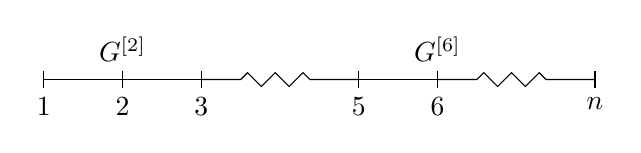
\begin{tikzpicture}[snake=zigzag, line before snake = 5mm, line after snake = 5mm]
    % draw horizontal line
    \draw (0,0) -- (2,0);
    \draw[snake] (2,0) -- (4,0);
    \draw (4,0) -- (5,0);
    \draw[snake] (5,0) -- (7,0);

    % draw vertical lines
    \foreach \x in {0,1,2,4,5,7}
      \draw (\x cm,3pt) -- (\x cm,-3pt);

    % draw nodes
    \draw (0,0) node[below=3pt] {$ 1 $} node[above=3pt] {$   $};
    \draw (1,0) node[below=3pt] {$ 2 $} node[above=3pt] {$ G^{[2]} $};
    \draw (2,0) node[below=3pt] {$ 3 $} node[above=3pt] {$  $};
    \draw (3,0) node[below=3pt] {$  $} node[above=3pt] {$  $};
    \draw (4,0) node[below=3pt] {$ 5 $} node[above=3pt] {$  $};
    \draw (5,0) node[below=3pt] {$ 6 $} node[above=3pt] {$ G^{[6]}$};
    \draw (6,0) node[below=3pt] {$  $} node[above=3pt] {$  $};
    \draw (7,0) node[below=3pt] {$ n $} node[above=3pt] {$ $};
  \end{tikzpicture}
\end{center}
Our model is the same as that of Tang et al. \cite{tmml10} though they
use slightly different notation.
Grindrod et al.'s model  \cite{gphe11} \cite{grihig13} is very similar to ours,
where an evolving graph is considered as a sequence of adjacency matrices.
Our model can also be seen as a special case of
the multi-layer networks discussed by Kivel{\"a} et al. \cite{kabg14}, where
there is only one set of layers for time.
% We present a preliminary discussion of using the model to mine citation networks.

% why BFS is important?

% Given a graph and a source node $s$,
% the breadth-first search (BFS) systematically discover every node that is reachable from $s$.
% As the name suggested, BFS expands the frontier of discovered regions
% uniformly across the breadth, i.e., the algorithm discovers all nodes
% that are $k$ walks away from $s$ before discovering any nodes that are
% $k+1$ walks away.
A temporal path is the basic element to
 define almost  all important evolving graph algorithms.
Matrix-matrix multiplication between consecutive adjacency matrices
were commonly used as a means of determining temporal paths \cite{gphe11,grihig13}. However, we show
in one specific case it fails to include all the temporal paths and thus should not be used
for searching evolving graphs in general.

Breadth-first search is probably the most basic graph searching algorithm and
it is also the building block of other graph algorithms like minimum spanning tree
and shortest path \cite{ckrs09}.
Despite the fact that graph metrics \cite{ntmm13,tmml09,tsmm09} and
various centrality measures like Katz centrality~\cite{gphe11,grihig13},
betweenness \cite{alhi15}, and closeness \cite{tmml10})
have been generalized for evolving graphs,
a BFS for evolving graphs, which we shall call it \emph{evolving-graph BFS},
was never explicitly described or verified.


In this paper,  we present descriptions of an evolving-graph BFS algorithm, but its main concern is with its sparse matrix
representation and linear algebraic computations.
We prove that the two algorithms (graph notation and algebra notation) are equivalent.

% GraphBlas related ideas

% This paper is organized as follows. The evolving-graph BFS algorithm is described
% and analyzed using graph notation in Section \ref{sec:breadth-first-search}. Section \ref{sec:evolv-graph-algor} considers the algebraic representation of the algorithm:
% A sparse matrix representation
% of an evolving graph is presented in \ref{sec:representation}.
% The algorithm is presented in \ref{sec:breadth-first-search-1} and
% the properties of the search tree is discussed in \ref{sec:short-temp-path}.
% The connection between a temporal path and a matrix-matrix multiplication is considered and discussed in \ref{sec:matr-matr-mult}. Finally,
% an application of the evolving-graph BFS in mining citation networks is described in Section \ref{sec:applications}.

\section{Breadth-First Search for Evolving Graphs}
\label{sec:breadth-first-search}

\subsection{Evolving-Graph BFS}
\label{sec:evolving-graph-bfs}

\begin{figure}[h]
 \begin{center}
    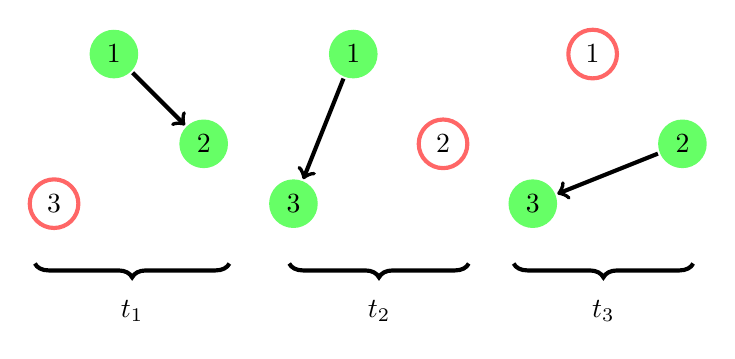
\begin{tikzpicture}[scale=.38, line width =1.5pt]
  \node[circle,fill=green1, minimum size=0.2cm] (n7) at (-5,7) {2};
  \node[circle,draw=red1, minimum size=0.2cm] (n8) at (-10,5) {3};
  \node[circle,fill=green1, minimum size=0.2cm] (n10) at (-8,10) {1};

  \node[circle,draw=red1, minimum size=0.2cm] (n6) at (3,7) {2};
  \node[circle,fill=green1, minimum size=0.2cm] (n4) at (-2,5) {3};
  \node[circle,fill=green1, minimum size=0.2cm] (n1) at (0,10) {1};

   \node[circle,fill=green1, minimum size=0.2cm] (n11) at (11,7) {2};
  \node[circle,fill=green1, minimum size=0.2cm] (n12) at (6,5)  {3};
  \node[circle,draw=red1, minimum size=0.2cm] (n14) at (8,10) {1};

  \foreach \from/\to in {n10/n7, n1/n4, n11/n12}
   \draw[every edge,->] (\from) -- (\to);
\draw [decorate,decoration={brace,amplitude=5pt},xshift=-4pt,yshift=0pt]
(4,3) -- (-2,3) node [midway,yshift=-0.6cm]{ $t_2$};
\draw [decorate,decoration={brace,amplitude=5pt},xshift=-4pt,yshift=0pt]
(-4,3) -- (-10.5,3) node [midway,yshift=-0.6cm]{ $t_1$};
\draw [decorate,decoration={brace,amplitude=5pt},xshift=-4pt,yshift=0pt]
(11.5,3) -- (5.5,3) node [midway,yshift=-0.6cm]{ $t_3$};
    \end{tikzpicture}
\end{center}
\caption{An evolving graph with 3 time stamps $t_1$, $t_2$ and $t_3$.
At each time stamp, the evolving graph is represented as a graph.
The green filled nodes in the figure are active nodes.}
\label{fig:eg_shortest_path}
\end{figure}

We show a small evolving graph $ \langle G^{[1]}, G^{[2]}, G^{[3]}\rangle$ with $3$ time stamps $t_1$, $t_2$ and $t_3$
in Figure \ref{fig:eg_shortest_path}, where each $G^{[i]}$ is a graph at time stamp $t_i$.
For example,
at time stamp $t_1$, the graph $G^{[1]}$ contains three nodes $1$, $2$ and $3$ and $(1,2)$ is an edge of $G^{[1]}$.
Though Figure \ref{fig:eg_shortest_path} presents a
directed evolving graph,  the algorithms that we shall discuss work on both
directed and undirected evolving graphs.
We shall use this example throughout the paper to illustrate various
notions.

Formally, an evolving graph $G_n $ is defined to be a sequence of graphs $\langle G^{[1]}, G^{[2]}, \ldots, G^{[n]}\rangle$,  where each $G^{[t]} = (V^{[t]}, E^{[t]})$ represents a graph at time stamp $t$.
We shall use the notation $(v, t)$ to represent
a node $v$ at time stamp $t$.
We say two nodes are \emph{connected} if there is an edge between them
and we say a node $(v,t)$ is \emph{active}, if $v$ is connected to at least a node other than itself at time stamp $t$. Otherwise we say it is \emph{inactive}.
In Figure \ref{fig:eg_shortest_path}, node $(1,t_1)$ and $(2,t_2)$  are active but node $(3,t_1)$ is inactive.

In order to define the evolving-graph BFS, we need the concept of a
\emph{temporal path}.
A temporal path on an evolving graph $G_n$ is a sequence of node-time stamp
pair $\langle (v_1, t_1), (v_2, t_2), \ldots, (v_m, t_m) \rangle$ such that
$t_1 \leq t_2 \leq \cdots \leq t_m$ and $v_i = v_j$ if and only if
$t_i \ne t_j$. The length of a temporal path is the length of the sequence.
For example, $\langle (1, t_1), (1, t_2), (3, t_2), (3, t_3) \rangle$ and
$\langle (1, t_1), (2, t_1), (2, t_3), (3, t_3) \rangle$
are two temporal paths from $(1, t_1)$ to $(3, t_3)$
on the evolving graph in Figure \ref{fig:eg_shortest_path}.

We would like a BFS on evolving graphs to work similar to that on graphs: the search starts with some source node $(s,t)$, called \emph{root}. It constructs a tree through discovering all nodes that are reachable by
temporal paths of length $k$ before moving to all nodes that are reachable by
 temporal paths of length $k+1$.
By construction, the time stamp of an active node is always not later than
that of its descendant. Suppose we
start with node $(1, t_1)$ in Figure \ref{fig:eg_shortest_path}.
After $1$ temporal path from $(1, t_1)$, we can reach
$(2, t_1)$ and $(1, t_2)$. After $2$ temporal paths, we can reach
$(2, t_1), (1, t_2), (2, t_2)$ and $(3, t_2)$.
% This example motivates us to define the reachable set of
% a node-timestamp pair.
Formally, we define the \emph{forward-neighbors} of a node $(v, t)$ to
be the set of all the reachable nodes after $1$ temporal path from
$(v, t)$, i.e., the nodes pointed by $v$ at time stamp $t$ and
the active node $v$ itself at later time stamps. In Figure
\ref{fig:eg_shortest_path},
the forward-neighbors of $(1, t_1)$  are $(2, t_1)$ and $(1, t_2)$ and
the forward-neighbors of $(2, t_1)$ is $(2, t_3)$.
See Algorithm  \ref{alg:bfs} for the evolving-graph BFS algorithm.

\begin{algorithm}[h]
 \SetKwFor{For}{for}{}{end}
 \SetKwFor{While}{while}{}{end}
 \SetKwFor{If}{if}{}{end}
 \SetKwFunction{nei}{forward-neighbors}
 \SetKwFunction{enqueue}{enqueue}
 \SetKwProg{Fn}{function}{}{end}
 \Fn{BFS($G_n, (s,t)$)}{
  $dict.(s,t) = 0$ \\
  $i = 1$ \\
  $fronter = \emptyset$ \\
  \enqueue{$frontier, (s,t)$} \\
 \While{$frontier \ne \emptyset$}{
   $next = \emptyset$ \\
   \For{$(u,t') \in frontier$}{
     \For{$(v,t'') \in$\nei{$(u,t')$}}{
          \If{$(v,t'') \notin d$}{
              $dict.(v,t'') = i$\\
              \enqueue{$next, (v,t'')$}
              }
         }
       }
  $frontier = next$ \\
  $i = i+1$ \\
  }
  \textbf{return} $dict$
}
 \caption{Evolving-graph BFS.
Let $G_n$ be an
evolving graph represented by adjacency lists and $(s, t)$ is a node
of $G_n$.
For each node-time stamp pair $(v_i,t_i)$,
we use a dictionary $dict.(v_i,t_i)$ to store its distance (the length of temporal
paths) from $(s, t)$. We also use
two first-in, first-out queue $frontier$ and $next$, where $frontier$
stores the frontier nodes of the current discovered regions and $next$ stores
the frontier nodes of the next level.
The algorithm returns $dict$ which stores all reachable node-time stamp pairs from $(s,t)$ such that if $dict.(v_i, t_i) = k$,
the length of the shortest temporal path
from $(s,t)$ to $(v_i, t_i)$ is $k$.}
 \label{alg:bfs}
\end{algorithm}

%Also need to consider the operations for matrix lists.

\subsection{Algebraic Evolving-Graph BFS}
\label{sec:representation}
As before, let $G_n = \langle G^{[1]}, G^{[2]}, \ldots, G^{[n]}\rangle$ be an evolving graph with $n$ time stamps. For each graph $G^{[t]}$, we use $A^{[t]}$ to denote
the corresponding adjacency matrix.
\[
A^{[t]}(i,j) =
\begin{cases}
 1 & \mbox{if $(i,j)$ is an edge of $G^{[t]}$,} \\
 0 & \mbox{otherwise.}
\end{cases}
\]
 Each $A^{[t]}$ can be represented by
a $|V|\times |V|$ sparse matrix,
where $|V|$ is the total number of nodes in $G_n$.
We use a sequence of adjacency matrices $A_n = \langle A^{[1]}, A^{[2]}, \ldots, A^{n]}\rangle$ to represent $G_n$.
For example, the evolving graph in Figure \ref{fig:eg_shortest_path}
can be represented as
\[
\Big\langle
  \begin{bmatrix}
    0 & 1 & 0 \\
    0 & 0 & 0 \\
    0 & 0 & 0
  \end{bmatrix},~
 \begin{bmatrix}
   0 & 0 & 1 \\
   0 & 0 & 0 \\
   0 & 0 & 0
 \end{bmatrix},~
 \begin{bmatrix}
  0 & 0 & 0 \\
  0 & 0 & 1 \\
  0 & 0 & 0
 \end{bmatrix}
\Big\rangle
\]


This algebraic formulation exploits a graphical interpretation of matrix--vector
products involving the adjacency matrix~\cite{kegi11}.
Let $G = (V, E)$ be a (directed or undirected) graph
and $k$ be a node in the graph $G$. If $A$ is the adjacency matrix of $G$ and
$b$ is the column vector
\[
b_i =
\begin{cases}
1 & \mbox{if $i = k$,} \\
0 & \mbox{otherwise,}
\end{cases}
\]
then $A^Tb$ is a column vector whose nonzero entries have indices that are the
forward-neighbors of $k$.

The evolving graph BFS can be thought of as a generalization of blocked
matrix--vector products.
Introduce a new operator $\odot$, a variation on the ordinary matrix--vector
product such that
\[
A^T \odot b =
\begin{cases}
b & \mbox{if $A^Tb \ne 0$,} \\
0 & \mbox{otherwise.}
\end{cases}
\]
Then, the forward-neighbors of node $(k, 1)$ in $A_n = \langle A^{[1]}, A^{[2]}, \ldots, A^{n]}\rangle$ are the nonzero indices of the
elements in the sequence
\begin{equation}
\label{eq:out_ne}
\big\langle (A^{[1]})^Tb, \quad  (A^{[2]})^T\odot b, \quad \ldots \quad (A^{[n]})^T\odot b \big\rangle.
\end{equation}
The forward-neighbors at time stamp $t$ are the nonzero indices of the $t$-th element of the above sequence.
Hence given $A_n$ and a vector $b$, we can use \eqref{eq:out_ne} to
get a $1$-step BFS tree. In Figure \ref{fig:eg_shortest_path}, the forward-neighbors
of node $(1, t_1)$ can be computed by

\begin{align*}
\left\langle
  \begin{bmatrix}
    0 & 0 & 0 \\
    1 & 0 & 0 \\
    0 & 0 & 0
  \end{bmatrix}\!\!\!\!
\begin{bmatrix}
1 \\
0 \\
0
\end{bmatrix}
,
 \begin{bmatrix}
   0 & 0 & 0 \\
   0 & 0 & 0 \\
   1 & 0 & 0
 \end{bmatrix}\!\!
\odot\!\!
\begin{bmatrix}
1 \\
0 \\
0
\end{bmatrix}
,
 \begin{bmatrix}
  0 & 0 & 0 \\
  0 & 0 & 0 \\
  0 & 1 & 0
 \end{bmatrix}\!\!
\odot\!\!
\begin{bmatrix}
1 \\
0 \\
0
\end{bmatrix}
\right\rangle
\\
=
\left\langle
\begin{bmatrix}
0 \\
1 \\
0
\end{bmatrix},~
\begin{bmatrix}
1 \\
0 \\
0
\end{bmatrix},~
\begin{bmatrix}
0 \\
0 \\
0
\end{bmatrix}
\right\rangle
\end{align*}
This means node $(2,t_1)$ and $(1,t_2)$ are the forward-neighbors of $(1,t_1)$.

Let $(A^{[i]})^Tb = c_i$.
At the second step, we need to compute the following components
\begin{align}
  \label{eq:5}
 \big\langle (A^{[1]})^Tc_1,   (A^{[2]})^T\odot c_1, \ldots,  (A^{[n]})^T\odot c_1  \big\rangle  \\
\big\langle (A^{[2]})^Tc_{2}, \ldots, (A^{[n]})^T\odot c_{2} \big\rangle \\
 \ldots  \\
  \big\langle (A^{[n]})^Tc_n \big\rangle
\label{eq:6}
\end{align}
If we sum these resulting vectors according to time stamps, we obtain
the forward-neighbors of the nodes computed at step $1$.
For $n =2$, we have
\[
\Big\langle
(A^{[1]})^Tc_1,~
(A^{[2]})^T\odot c_1 + (A^{[2]})^T c_2
\Big\rangle.
\]
If we form a block triangular matrix $\bm{A_n}^T$
\[
\bm{A_n}^T =
\begin{bmatrix}
(A^{[1]})^T &   0            & \cdots  &  & 0 \\
\sigma(A^{[2]})^T & (A^{[2]})^T & 0         &\cdots  & \vdots \\
\sigma(A^{[3]})^T & \sigma(A^{[3]})^T & (A^{[3]})^T & \cdots \\
   \vdots              &                              &      \vdots            &  &  \vdots \\
\sigma(A^{[n]})^T &                  &       \cdots                      &  & (A^{[n]})^T
\end{bmatrix},
\]
where  $\sigma(A^{[i]})^Tb = (A^{[i]})^T\odot b$, and a block vector $\bm{b}$
\[
\bm{b}^T = [b^T, 0, \cdots, 0  ],
\]
then \eqref{eq:out_ne} is equivalent to $\bm{A_n}^T\bm{b}$ and
summing \eqref{eq:5}-\eqref{eq:6} is equivalent to $\bm{A_n}^T(\bm{A_n}^T\bm{b})$.
In general, we can define an evolving-graph BFS using
block vector-matrix multiplications. The algorithm is presented in Algorithm
\ref{alg:bfsla}.

\begin{algorithm}[h]
 \SetKwFor{For}{for}{}{end}
 \SetKwFor{While}{while}{}{end}
 \SetKwFor{If}{if}{}{end}
 \SetKwFunction{nei}{forward-neighbors}
 \SetKwFunction{enqueue}{enqueue}
 \SetKwFunction{nz}{nonzeros}
 \SetKwFunction{intersect}{intersect}
 \SetKwFunction{map}{map}
 \SetKwProg{Fn}{function}{}{end}
 \Fn{ABFS($A_n, (s,t)$)}{
   Form $\bm{A}^T$ from $A_n$\\
   $m = A^{[1]}.dimension$ \\
   $b$ is a sparse vector of length $mn$ \\
   $b(s+mt) =1$ \\
   $i = 1$ \\
   $dict.(s,t) = 0$ \\
   \While{\nz{$b$} $\ne \emptyset$}{
       $\bm{b} = \bm{A}^T\bm{b}$ \\
       \For{$i$ in \nz{$b$}}{
         $node =$ \map{$i$} \\
         \If{$node$ in $dict$}{
           $b(i) = 0$ \\
         }
      }
      $nodes =$\map{$b$}\\
       \For{$node$ in $nodes$}{
           $dict.node = i$
         }

       $i = i + 1$
       }
  \textbf{return} $dict$ \\
}
 \caption{Algebraic evolving-graph BFS.
Let $A_n$ be the corresponding adjacency matrices of $G_n$ and
$(s,t)$ a node of $G_n$. As in Algorithm \ref{alg:bfs}, we use a dictionary $dict.(v_i, t_i)$
to store $(v_i, t_i)$'s distance from $(s,t)$. Function \texttt{nonzeros(v)}
returns the nonzero indices of a given vector  $v$ and function \texttt{map(b)}
maps a block vector's indices to their corresponding nodes. The algorithm  returns
$dict$ which stores all the reachable active nodes and their distance from $(s,t)$.}
 \label{alg:bfsla}
\end{algorithm}

Representing evolving graphs as sparse matrices offers great flexibility
on the search direction. If we define the \emph{backward-neighbors} of a
node $(v,t)$ to be a set of nodes that precede $(v,t)$ if we travel backwards
in time. Then the backward-neighbors of $(v,t)$ can be computed by
\begin{equation}
\label{eq:backward}
(A^{[t]})b + (A^{[t+1]})\odot b + \cdots + (A^{[n]})\odot b.
\end{equation}
We shall get a backward traversal algorithm if we replace
the vector-matrix multiplication $\bm{A_n}^T\bm{b}$
by $\bm{A_n}\bm{b}$, where
\[
\bm{A_n} =
\begin{bmatrix}
A^{[1]} &   0            & \cdots  &  & 0 \\
\sigma(A^{[2]}) & A^{[2]} & 0         &\cdots  & \vdots \\
\sigma(A^{[3]}) & \sigma(A^{[3]}) & A^{[3]} & \cdots \\
   \vdots              &                              &      \vdots            &  &  \vdots \\
\sigma(A^{[n]}) &                  &       \cdots                      &  & A^{[n]}
\end{bmatrix}.
\]
Having the ability to traverse backwards is important for many real-life applications.
We shall show an example in Section \ref{sec:applications}.

Algorithm \ref{alg:bfsla} outlines the basic idea of an algebraic evolving-graph BFS.
But in practice we don't need to form $\bm{A}$ and $\bm{b}$ explicitly at step $4$ and $6$. By realizing the dependency between these sparse matrices,
we can compute  the result in parallel.

\subsection{Analysis}
\label{sec:analysis}

% adjacency matrices
Suppose $G_n$ is represented by adjacency lists.
Then the number of adjacency lists is the same as the number
of active nodes in $G_n$. So for large $n$, this representation
can use a large amount of memory.
For the graph $G^{[i]} = (V^{[i]}, E^{[i]})$ at time stamp $i$,
we denote the active node set of $V^{[i]}$ as $\tilde V^{[i]}$,
where we have $\tilde V^{[i]} \subseteq V^{[i]}$.
Step $10$ of  Algorithm \ref{alg:bfs} ensures each active node-time stamp pair in $G_n$ is enqueued in $next$ (and then $frontier$) at most once.
And so \texttt{forward-neighbors} loops through each
active node-time stamp pair at most once.
The operations of enqueuing take $O(1)$ time.
Thus the total operations of enqueuing are
$O(\sum_{i=1}^n|\tilde V^{[i]}|)$, where $|\cdot|$ represents the number of elements of a set.  Let $\sum_i |\tilde V^{[i]}| = |\tilde V|$ and $\sum_i |E^{[i]}| = |\hat E|$.
Then the time of scanning
\texttt{forward-neighbors} is
\[
\sum_{i=1}^n\sum_{v \in \tilde V^{[i]}} \texttt{forward-neighbors}(v) =
O(|\hat E|),
\]
by the definition of forward-neighbors.
Hence the total running time is $O(|\hat E|+ |\tilde V|)$.

\begin{thm}[Correctness of evolving-graph BFS]
Let an evolving graph $G_n$ and a starting node $(s,t_0)$ be given.
The evolving-graph BFS discovers every active node that is reachable from the source $(s,t_0)$ and $d.(v, t)$ is the length of the shortest temporal path
from $(s,t_0)$ to $(v,t)$.
\end{thm}
\proof
We could map an evolving graph $G_n$ to a static graph $G$ in such a way that
if there is an edge from $(v, t)$ to $(u,t)$ in $G_n$, there is an edge from $v_t$ to $u_t$ in $G$.
For any two nodes $v_s$ and $v_t$ in $G$,  if $s < t$, we add an edge from $v_s$ to $v_t$.
By construction, the forward-neighbors of an active node $(v, t)$ in $G_n$
are in one-to-one correspondence with the forward-neighbors of a node $v_t$ in $G$.
Hence the correctness of the evolving graph BFS follows from that of a static graph.
\endproof

\begin{thm}
 Algorithm \ref{alg:bfs} and Algorithm \ref{alg:bfsla} are equivalent.
\end{thm}
\proof
We shall check the two algorithms are equivalent in each module of
the method.
The initialization steps are trivially equivalent.
By the construction of $\bm{A^T}$,
step $9$ of Algorithm \ref{alg:bfsla} computes the forward-neighbors
of all the frontier nodes, which is equivalent to step $8$-$9$
of Algorithm \ref{alg:bfs}. Step $10$-$15$ of Algorithm \ref{alg:bfsla} ensures
active nodes will not be visited twice, which is equivalent to step $10$
of Algorithm \ref{alg:bfs}. Finally, a dictionary $dict$ is used in both algorithms
to keep record of the distance of each node from the source $(s,t)$.
\endproof


\subsection{Search Tree}
\label{sec:short-temp-path}

We say two nodes $(v_1,t_1)$ and $(v2, t_2)$ are \emph{temporally connected} if
$(v_1, t_1)$ and $(v2,t_2)$ are connected by a temporal path.
Notice this notion is symmetric, reflexive but not transitive. For example, suppose
$t_1 < t_2 < t_3$ and $(v_1, t_1)$ and $(v_3, t_3)$ are temporally connected
by a temporal path from $(v_1,t_1)$ to $(v_3, t_3)$. Also
$(v_3, t_3)$ and $(v_2, t_2)$ are temporally connected by a temporal path from
$(v_2,t_2)$ to $(v_3, t_3)$. But this does not imply $(v_1, t_1)$ and $(v_2, t_2)$ are temporal connected.

Given a root node $(s, t)$, during the execution the BFS discussed above builds a search tree, denoted by $T(s,t)$,
where nodes are temporally connected.
\begin{lemma}
For a node active at different time stamps, say $(s, t_1)$ and $(s,t_2)$ such that $t_1 < t_2$,  we have $T(s, t_2) \subseteq T(s, t_1)$.
\end{lemma}
\proof
Suppose $(v, t)$ belongs to $T(s, t_2)$. Then there exists an temporal path
(constructed by the evolving graph BFS) from $(s,t_2)$ to $(v,t)$. Since both
$(s,t_1)$ and $(s,t_2)$ are active, $(s,t_2)$ is an out-neighbor of $(s,t_1)$ by definition, i.e., there exists an edge from $(s,t_1)$ to $(s,t_2)$.  Hence there exists a temporal path
from $(s,t_1)$ to $(v,t)$ and so $(v,t) \in T(s,t_1)$.
\endproof

% consider $(A+I)^Tb$, which records all the connected components.
% consider the huge matrix block and how to relate it.

% \subsection{Online Searching}
% \label{sec:online-searching}

% In this section, we consider ways of  updating new graphs. Suppose $A_n $ is
% an evolving graph with $n$ timestamps. We received a new graph $A^{[n+1]}$
% at timestamp $n+1$. How to update the tree components while minimize the computation?
% The forward-neighbors at timestamp $$

\section{Node Activeness and its Impact}
\label{sec:matr-matr-mult}

\subsection{Aggregated Graphs}
\label{sec:aggregated-graphs}

In this section, we answer the question why we need evolving graph.

At the beginning of the paper, we set up a game played by three people $A$, $B$,
and $C$ and we showed if


\subsection{Temporal Path}
\label{sec:temporal-path}

In this subsection, we compare with the ``wrong'' way of traveling an evolving graph
and show the importance of node activeness.


\subsection{Matrix-Matrix Multiplication}
\label{sec:matr-matr-mult-1}

For adjacency matrices $A^{[s]}$ and $A^{[t]}$, where $s < t$, a nonzero entry
$(i,j)$ of $A^{[s]} A^{[t]}$ indicates a temporal path from $(i,s)$ to $(j,t)$ via
some node $k$.
In general, a nonzero entry $(i,j)$ of the matrix $A^{[1]}A^{[2]}\cdots A^{[n]}$
indicates a temporal path $p$ that starts at $(i,1)$ and ends at  $(j,n)$.
Notice $p$ must go through at least one edge at each time stamp between $1$ and $n$.
For the evolving graph in Figure \ref{fig:eg_shortest_path}, $A^{[1]}A^{[2]}$
is a zero matrix since there is no temporal path from time stamp $t_1$ to $t_2$ that
go through at least one edge at $t_1$. However,
$\langle(1, t_1), (1, t_2), (3,t_2)\rangle$ is a temporal path of Figure \ref{fig:eg_shortest_path}.

Introducing ones on the diagonal of the matrices will still get the wrong result.

% But it provides no information about the nodes in between. In addition, the temporal path must pass at least
%  one node at each timestamps. We believe this requirement is too restrictive. For example,
% $A^{[t_1]}A^{[t_2]}A^{[t_3]}$ is a zero matrix. Let $\langle i,j,\ldots k \rangle$ represents the sets of all possible subsets of $\langle 1, 2, \ldots, n \rangle$, where $i<j<\cdots<k$, then
% the nonzero entries of the matrix
% \[
% \sum_{i,j,\ldots,k}A^{[1]}A^{[i]}A^{[j]}\cdots A^{[k]}A^{[n]},
% \]
% indicates temporal paths  from temporal paths from timestamp $1$ to $n$.

\section{Implementation in Julia}
\label{sec:implementation-julia}

In order to study evolving graphs and experiment with various graph types, we have developed EvolvingGraphs.jl  \cite{zhang15}, a software package in the Julia language \cite{bkse12} for the creation, manipulation, and study of dynamic networks.
Julia is a high-level, high-performance dynamic programming language for technical
computing. When we implement EvolvingGraphs.jl, we make particular use of
the parameterizable type system and multiple dispatch in Julia.
We define a data type  \texttt{MatrixList}, which represents an evolving graph
as a sequence of sparse matrices stored in compressed sparse column (CSC) format.
Many basic graph functions are defined for \texttt{MatrixList}, including
retrieving nodes, time stamps, and matrices.

\section{Application to Citation Networks}
\label{sec:applications}

We shall map a database of research papers to an evolving graph $G_n$
in such a way that if author $i$ cited author $j$ on a paper published
at  time $t$, the evolving graph $G_n$ contains a directed edge from
$i$ to $j$ at time stamp $t$. Then given an author $a$ at time stamp $t_0$,
we can use our evolving-graph BFS to construct $T(a, t_0)$ which is
a set of all the authors that have been influenced by $a$'s work at
time $t_0$. We define a \emph{community} to be a group of
researchers that share the same information source.
For example, given a paper published by $a$ at year $2016$,
we can determine $a$'s community by first backward searching to
find the source then forward searching to find the descendants.

To design such system, we shall use two parameters:
 a parameter for
determining the layers of the backward search tree which can be chosen by the user;
a second parameter for determining the number of roots as a means of
filtering out unessential or overlapping trees. The subset of roots can be determined
by ranking algorithms like PageRank or machine-learning based preference ranking.


\section{Conclusion}

In this paper, we have introduced and analyzed the evolving-graph BFS in both
graph and algebraic notation.
This paper leaves important extensions open for further research. First, it is
of interest to extend the evolving-graph BFS algorithm for weighted evolving graphs, which can provide more valuable information when the degree of connectivity is available in the data.
Second, efficient algebraic representations and algorithms need to be addressed.
One major advantage of representing evolving graphs as sparse matrices
is the matrix representation is highly structured so it is easy to design
high performance parallel implementations.
Third, depth-first search and other graph traversal algorithms can be
extended for searching evolving graphs using similar ideas.


% % use section* for acknowledgement
% \section*{Acknowledgment}


% The authors would like to thank...
% more thanks here


% trigger a \newpage just before the given reference
% number - used to balance the columns on the last page
% adjust value as needed - may need to be readjusted if
% the document is modified later
%\IEEEtriggeratref{8}
% The "triggered" command can be changed if desired:
%\IEEEtriggercmd{\enlargethispage{-5in}}

% references section

% can use a bibliography generated by BibTeX as a .bbl file
% BibTeX documentation can be easily obtained at:
% http://www.ctan.org/tex-archive/biblio/bibtex/contrib/doc/
% The IEEEtran BibTeX style support page is at:
% http://www.michaelshell.org/tex/ieeetran/bibtex/
%\bibliographystyle{IEEEtran}
% argument is your BibTeX string definitions and bibliography database(s)
%\bibliography{IEEEabrv,../bib/paper}
%
% <OR> manually copy in the resultant .bbl file
% set second argument of \begin to the number of references
% (used to reserve space for the reference number labels box)

\bibliographystyle{myplain2-doi}

\bibliography{strings,njhigham,paper}

% that's all folks
\end{document}
